\documentclass[11pt]{article}

\usepackage[margin=1in]{geometry}
\usepackage{booktabs}
\usepackage{graphicx}
\usepackage{hyperref}
\usepackage{xcolor}
\usepackage{caption}
\usepackage{array}
\usepackage{amsmath}
\usepackage{enumitem}
\usepackage{fancyhdr}
\usepackage[T1]{fontenc}

\hypersetup{
    colorlinks=true,
    linkcolor=blue,
    urlcolor=blue,
    citecolor=blue
}

\pagestyle{fancy}
\fancyhf{}
\fancyhead[L]{HLS-Eval Reproduction + One Year Later}
\fancyhead[R]{\thepage}
\renewcommand{\headrulewidth}{0.4pt}

\newcommand{\code}[1]{\texttt{#1}}

\title{\textbf{HLS-Eval Reproduction and Extension:\\
A One-Year-Later Evaluation of LLMs for HLS Code Generation}}
\author{Michael Incorvaia}
\date{August 12, 2026}

\begin{document}

\maketitle

\begin{abstract}
We reproduce the zero-shot HLS kernel generation baseline from
\emph{HLS-Eval: A Benchmark and Framework for Evaluating LLMs on
High-Level Synthesis Design Tasks} (Abi-Karam \& Hao, ICLAD 2025), and
extend it with three language models released after the paper. Using
the paper's original harness with a Vitis-free compilation backend, we
evaluate four models across 57 designs drawn from the PolyBench,
MachSuite, and C2HLSC suites, scoring three of the paper's four staged
metrics (parseable, compilable, runnable) with bootstrap confidence
intervals. Our reproduction of the DeepSeek-V3 anchor shows a
substantial gap at pass@1 (46.3\% vs.\ the paper's 63.3\%) that nearly
closes at pass@5 (63.2\% vs.\ 65.9\%), which we trace to a fixed
\code{max\_tokens=8192} generation cap truncating a meaningful share of
completions rather than a genuine capability gap. Among the three
extension models, \code{qwen3-coder} clears 67.4\% pass@1 on the
runnable metric --- a 21-point improvement over the 2025 anchor under
identical harness conditions --- while a newer, more verbose model
(\code{deepseek-v4-pro}) underperforms the 2025 baseline, an artifact of
disproportionate exposure to the same token cap rather than reduced
capability. We report six additional infrastructure and reference-design
issues uncovered during this run, all independent of any language
model, and recommend three concrete follow-ups.
\end{abstract}

\tableofcontents

\section{What Was Reproduced}

We reproduce the zero-shot HLS generation task defined in the original
paper: given a natural-language kernel description, a header file, and a
testbench, the model generates a C++ implementation. We score three of
the paper's four staged metrics --- \textbf{parseable}, \textbf{compilable},
and \textbf{runnable} --- at $n_{\text{samples}}=5$, $T=0.7$, matching the
paper's sampling protocol. The fourth metric, \textbf{synthesizable}, is
out of scope: Vitis HLS is not installed on the evaluation machine, so
every synthesis cell is recorded as \emph{skipped}, not failed.

\textbf{Run provenance.} Repository \code{hls-eval} at commit
\code{adea9ff} (2026-07-30), \code{uv}-managed, evaluated 2026-08-12.
Compilation via a Vitis-free stock C-simulation backend
(\code{ext/stock\_tools.py}) using \code{clang++} 18.1.3 on Linux
6.6.87.2 (WSL2), Python 3.12.3.

\subsection{Scope}

57 designs across PolyBench, MachSuite, and C2HLSC --- the three suites
independently verified (prior to running any model) to compile and run
at 100\% under a stock compiler with no Xilinx software present. This is
3 short of the 60 designs counted in that verification pass; the
discrepancy was not chased down and is flagged here as an open, minor
gap rather than silently absorbed.

\subsection{Models}

\begin{table}[h]
\centering
\begin{tabular}{@{}llll@{}}
\toprule
\textbf{Role} & \textbf{Model} & \textbf{Provider} & \textbf{Notes} \\
\midrule
Anchor & \code{deepseek-chat-v3-0324} & OpenRouter (SiliconFlow) & Closest dated snapshot to the paper's \code{DeepSeek-V3} \\
Extension & \code{qwen3-coder} & OpenRouter & \\
Extension & \code{deepseek-v4-pro} & OpenRouter & \\
Extension & \code{qwen3-235b-a22b-thinking-2507} & OpenRouter & \\
Dropped anchor & \code{qwen-2.5-coder-32b-instruct} & --- & See \S\ref{sec:broke} \\
\bottomrule
\end{tabular}
\caption{Model roster. The alias \code{deepseek/deepseek-chat} was
deliberately avoided as the anchor ID: it is a moving alias that
resolves today to a v3.1/v3.2/v4-era model, which would silently anchor
the reproduction two generations later than the paper's run.}
\end{table}

\textbf{Deviation from the paper.} The paper used Together AI as its
sole inference provider. This run used OpenRouter, which load-balances
requests across multiple providers serving nominally identical weights
at potentially different quantizations. Numeric precision is therefore
an uncontrolled variable here in a way it was not for the paper (see
Table~\ref{tab:providers}).

A total of 1{,}140 LLM calls were made across the four-model roster;
2 provider-level errors occurred, both auto-recovered on retry, with
0 unrecovered failures.

\section{Reproduction Result: Paper's Numbers vs.\ Ours}

Table~\ref{tab:paper} reproduces the paper's published anchor results
(Table III of the original paper), evaluated across all 94 benchmark
designs with Vitis HLS synthesis included, using Together AI.

\begin{table}[h]
\centering
\begin{tabular}{@{}lcccccc@{}}
\toprule
\textbf{Model} & \textbf{parse@1} & \textbf{parse@5} & \textbf{compile@1} & \textbf{compile@5} & \textbf{run@1} & \textbf{run@5} \\
\midrule
DeepSeek V3 (paper) & 100.0\% & 100.0\% & 94.1\% & 97.6\% & \textbf{63.3\%} & \textbf{65.9\%} \\
Qwen2.5-Coder-32B (paper) & 95.5\% & 97.6\% & 90.8\% & 92.9\% & 57.6\% & 58.8\% \\
\bottomrule
\end{tabular}
\caption{Paper's original zero-shot generation results (Abi-Karam \&
Hao, 2025, Table III), 94-design benchmark, Together AI provider,
Vitis HLS 2024.1.}
\label{tab:paper}
\end{table}

Table~\ref{tab:mine} reports our reproduction under the conditions
described in \S1: 57-design subset, OpenRouter provider, no synthesis
metric, with bootstrap 95\% confidence intervals over designs (10{,}000
resamples).

\begin{table}[h]
\centering
\begin{tabular}{@{}lcccccc@{}}
\toprule
\textbf{Model} & \textbf{parse@1} & \textbf{parse@5} & \textbf{compile@1} & \textbf{compile@5} & \textbf{run@1} & \textbf{run@5} \\
\midrule
deepseek-chat-v3-0324 & 63.2\% & 87.7\% & 61.4\% & 86.0\% & 46.3\% & \textbf{63.2\%} \\
\emph{95\% CI} & \scriptsize{[54.0, 72.3]} & \scriptsize{[79.0, 94.7]} & \scriptsize{[52.3, 70.2]} & \scriptsize{[77.2, 94.7]} & \scriptsize{[35.8, 56.8]} & \scriptsize{[50.9, 75.4]} \\
\bottomrule
\end{tabular}
\caption{Our reproduction, 57-design subset, OpenRouter provider, no
synthesis. Bracketed values are 95\% bootstrap CIs over designs.}
\label{tab:mine}
\end{table}

\textbf{The pass@1 gap is real, but the pass@5 gap nearly vanishes}:
63.2\% versus the paper's reported 65.9\% on the metric that matters
most --- runnable, i.e., functional correctness. A model that recovers
almost fully by its fifth sample but stumbles on its first is the
signature of a \emph{budget or formatting} problem, not a capability
gap. Section~\ref{sec:broke} identifies the specific mechanism:
\code{max\_tokens=8192} truncates a meaningful share of completions
before the closing output tag, and a truncated sample counts as a hard
failure at $k=1$ even when the other four samples typically succeed.
The pass@1 numbers in Table~\ref{tab:mine} should be read as a
\textbf{lower bound} on model capability, not a clean apples-to-apples
comparison to the paper.

Three confounds prevent a fully clean comparison, stated plainly:

\begin{enumerate}[leftmargin=*]
\item \textbf{Different benchmark subset.} The paper's 94 designs vs.\
our 57 (CHStone and Rosetta excluded here for Xilinx-header and
missing-testbench reasons documented in \code{FINDINGS.md}).
\item \textbf{Different provider.} OpenRouter/SiliconFlow vs.\ Together
AI, with quantization unpinned in our run.
\item \textbf{\code{max\_tokens=8192}} was not part of the paper's
stated methodology and caps at least 21\% of all completions in this
run.
\end{enumerate}

\textbf{Qwen2.5-Coder-32B-Instruct was not reproduced.} This is the
paper's other anchor model. It was dropped from the roster
(\S\ref{sec:broke}) prior to the full sweep; its paper-reported numbers
in Table~\ref{tab:paper} are cited for reference only and are not
compared against any result from this run.

\section{One Year Later: The Extension}

\begin{table}[h]
\centering
\begin{tabular}{@{}lcccc@{}}
\toprule
\textbf{Model} & \textbf{parse@1} & \textbf{compile@1} & \textbf{run@1} & \textbf{run@5} \\
\midrule
deepseek-chat-v3-0324 (2025 anchor) & 63.2\% & 61.4\% & 46.3\% & 63.2\% \\
qwen3-235b-a22b-thinking-2507 & 73.7\% & 70.9\% & 52.3\% & 68.4\% \\
deepseek-v4-pro & 52.3\% & 49.5\% & 39.0\% & 61.4\% \\
\textbf{qwen3-coder} & \textbf{99.7\%} & \textbf{96.8\%} & \textbf{67.4\%} & \textbf{70.2\%} \\
\bottomrule
\end{tabular}
\caption{Extension results: three post-paper models compared against
the 2025 DeepSeek-V3 anchor, same harness and conditions. All values
pass@$k$, point estimates (see \code{results/aggregate.json} for full
95\% CIs).}
\label{tab:extension}
\end{table}

\textbf{\code{qwen3-coder} is the clear standout.} Its parse and compile
rates are both essentially saturated (99.7\%, 96.8\%), indicating the
harness or task itself --- not the model --- is now the bottleneck at
those two stages. Its run@1 (67.4\%) is 21 percentage points above the
2025 anchor under identical harness constraints, a defensible
"the gap closed" result.

\textbf{\code{deepseek-v4-pro} is the weakest model tested}, trailing
the 2025 anchor on every metric despite being the newer DeepSeek
release. This is very likely an artifact rather than a genuine
regression: it is one of the two models hit hardest by the
\code{max\_tokens} truncation described in \S\ref{sec:broke} --- its
no-code-extracted rate is 132/285 samples (46.3\%), the highest of any
model tested, with a combined parse-failure rate of 136/285 (47.7\%). A
verbose or reasoning-heavy model is punished disproportionately under a
fixed, small token budget; this result should not be read as evidence
that the newer model is less capable.

\textbf{Headline.} One year of model progress did not translate
uniformly into gains on this benchmark under a fixed
\code{max\_tokens=8192} ceiling --- the newest, most capable models
are, if anything, more exposed to that ceiling than the 2025 baseline
was.

\begin{figure}[h]
\centering
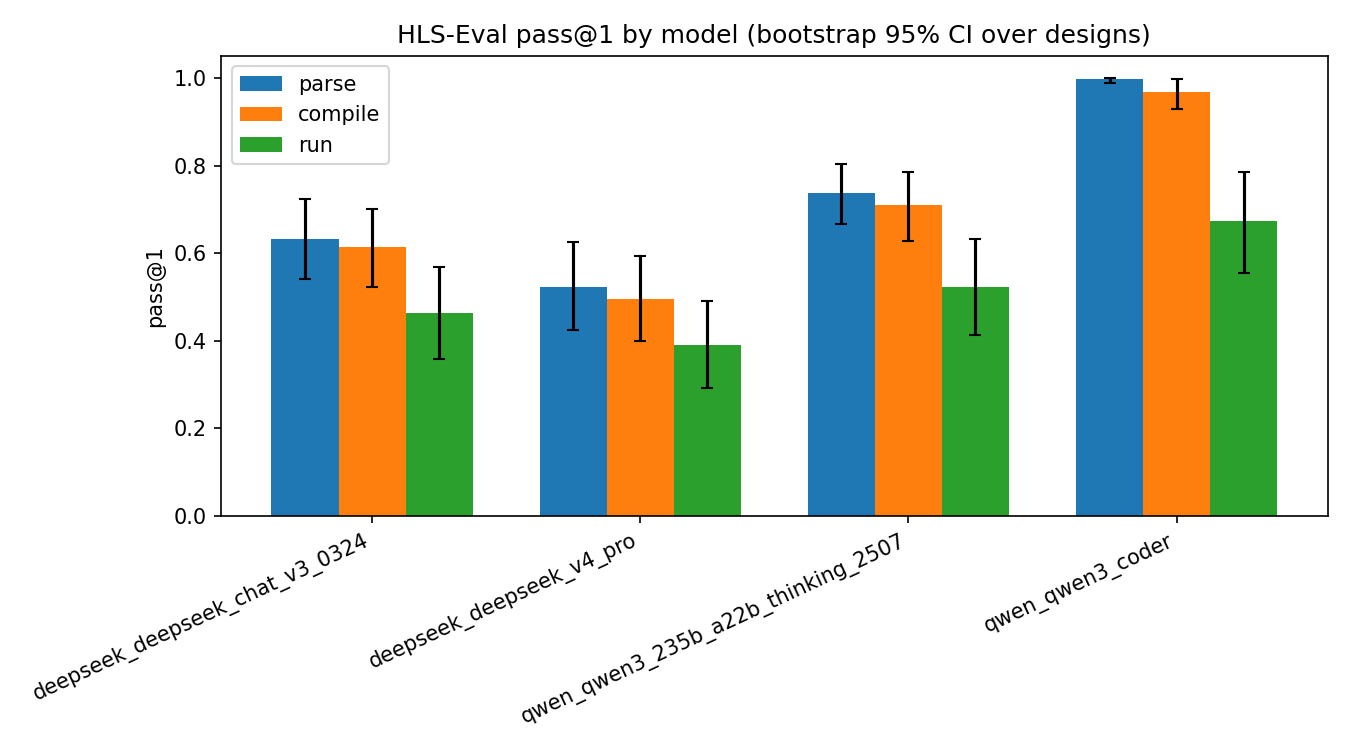
\includegraphics[width=0.85\textwidth]{../figures/repro_vs_paper.png}
\caption{Pass@1 by model and metric, with bootstrap 95\% confidence
intervals over designs.}
\label{fig:results}
\end{figure}

\section{What Broke}
\label{sec:broke}

Ordered roughly by how much each issue should change how the results
above are read.

\subsection{\code{max\_tokens=8192} truncates a meaningful share of completions}

Running \code{diagnose\_parse.py} over all 1{,}141 evaluations: 72.1\%
parsed cleanly, 27.0\% had no extractable code tags, and 0.9\% had
malformed tags. Of the entire run, 21.0\% of calls terminated with
\code{finish\_reason=length} --- the provider's own signal that
generation was cut off rather than completed. The diagnostic tool's own
output states:

\begin{quote}
\emph{`odd\_tags' usually means the response was cut off mid-code. That
is a property of the max-token setting in this run, not of the model's
HLS ability.}
\end{quote}

\begin{table}[h]
\centering
\begin{tabular}{@{}lcccc@{}}
\toprule
\textbf{Model} & \textbf{ok} & \textbf{no\_tags} & \textbf{odd\_tags} & \textbf{failure rate} \\
\midrule
qwen3-coder & 284 & 0 & 1 & 0.4\% \\
qwen3-235b-a22b-thinking-2507 & 210 & 72 & 3 & 26.3\% \\
deepseek-chat-v3-0324 & 180 & 104 & 1 & 36.8\% \\
deepseek-v4-pro & 149 & 132 & 4 & 47.7\% \\
\bottomrule
\end{tabular}
\caption{Per-model parseability breakdown from \code{diagnose\_parse.py}, 1{,}140 evaluations (frozen roster only).}
\end{table}

Not every failure is attributable to truncation: 318 total parse
failures vs.\ 240 calls terminated by \code{length} implies
approximately 78 failures completed normally
(\code{finish\_reason=stop}) and still failed to parse --- a genuine
format/extraction miss, distinct from the token-budget issue. Both
mechanisms are real and should not be conflated in a re-run.

\textbf{Recommended fix (not attempted here --- harness frozen once the
sweep started, per the run plan):} raise \code{max\_tokens} to roughly
12{,}000--16{,}000, especially for reasoning-tagged models, and re-run.
This is judged the single highest-value follow-up.

\subsection{The Qwen2.5-Coder-32B anchor could not be reproduced}

Every harness request to \code{qwen/qwen-2.5-coder-32b-instruct}
returned \code{finish\_reason: "error"} with corrupted output and
implausible token accounting (\code{prompt\_tokens: 0,
completion\_tokens: 1}), while a hand-written \code{curl} to the same
model and provider succeeded cleanly. A bisection script varied one
factor at a time --- prompt content/size, temperature, \code{max\_tokens},
streaming, SDK vs.\ raw HTTP transport --- and found every real-prompt
variant failed identically; only a short synthetic test prompt
succeeded. \textbf{Verdict:} the long, structured HLS-Eval prompt itself
breaks this specific model/provider/serving-stack combination; it is
not a parameter or SDK issue.

This model has exactly one OpenRouter provider (Cloudflare) with
unknown quantization and no failover. Given a fixed debugging timebox,
this was reported as a finding rather than pursued further:
\textbf{DeepSeek-V3 is the sole paper anchor in this run.} Testing
against Together AI (the paper's actual provider) is the natural next
step to isolate whether this is Cloudflare/OpenRouter-specific.

\subsection{Provider and quantization are uncontrolled variables}

\begin{table}[h]
\centering
\begin{tabular}{@{}llll@{}}
\toprule
\textbf{Model} & \textbf{OpenRouter providers} & \textbf{Quantization} & \textbf{Note} \\
\midrule
qwen-2.5-coder-32b & 1 (Cloudflare) & unknown & no failover \\
deepseek-chat-v3-0324 & 4 & bf16/fp4/fp8 & 88\% worst-case uptime \\
qwen3-coder & 5 & fp4/fp8/unknown & healthy \\
deepseek-v4-pro & 18 & fp4/fp8/unknown & 0.14\% worst-case uptime, one provider \\
qwen3-235b-thinking & 4 & fp8/unknown & healthy \\
\bottomrule
\end{tabular}
\caption{Preflight provider/quantization survey.}
\label{tab:providers}
\end{table}

The paper used a single inference provider. Reproducing an open-weights
benchmark through a routing layer means precision is uncontrolled, and
for one model, unknowable. This alone would explain a meaningful
fraction of any gap versus the paper's numbers even under an unlimited
token budget.

\subsection{Sweep pace}

Estimated at 1--2 hours, the sweep took 388.6 minutes ($\approx$6.5
hours) for 1{,}140 calls, attributable to reasoning-model latency (the
two thinking/verbose-tagged models dominate wall time). This is not a
defect, but is worth accounting for when scheduling a re-run.

\subsection{Reference-design and harness bugs}

Found prior to running any language model; full detail and reproduction
steps in \code{FINDINGS.md}.

\begin{itemize}[leftmargin=*]
\item 12 of 32 CHStone designs ship with no testbench --- the
\emph{runnable} metric is undefined for them, not failed. Scoring them
as failures would understate CHStone runnability by 37.5\%.
\item \code{flowgnn/fgnn\_linear}'s testbench calls \code{printf} with
no \code{<cstdio>} include --- builds under Vitis's bundled clang
(which pulls the header in transitively) but not under a standard
compiler.
\item \code{gnnbuilder/gather\_node\_neighbors}'s testbench writes out
of bounds and triggers a stack-smashing abort under GCC --- silent
under Vitis's clang, which does not enable the stack protector by
default.
\item The harness sets no execution timeout; a single generated
infinite loop hangs a worker for the remainder of a sweep.
\item Execution inherits the parent process's working directory; any
testbench performing relative-path file I/O reads from the wrong
location.
\end{itemize}

\subsection{The 57-vs-60-design gap}

The prior verification pass counted 60 clean designs across PolyBench,
MachSuite, and C2HLSC; the actual sweep manifest lists 57. This was not
investigated further and is logged here as an open, minor discrepancy.

\section{Recommended Next Steps}

\begin{enumerate}[leftmargin=*]
\item \textbf{Re-run with a larger \code{max\_tokens}} (12{,}000--16{,}000).
Cheap, and the single highest-leverage fix given how much of the
current gap traces to truncation rather than capability.
\item \textbf{Add a Together AI key} and re-test the Qwen2.5-Coder-32B
anchor on the paper's original provider, to isolate whether the
observed failure is OpenRouter/Cloudflare-specific or a genuine
harness/model interaction.
\item \textbf{Install Vitis HLS} (or a viable open-source synthesis
substitute) to restore the fourth metric and complete the 4-of-4 metric
comparison to the paper.
\item \textbf{Extend to CHStone and Rosetta} once the testbench-less
CHStone designs and the Xilinx-header dependency in Rosetta are
handled, to reach the paper's full 94-design scope.
\end{enumerate}

\section*{Appendix: Run Provenance}
\addcontentsline{toc}{section}{Appendix: Run Provenance}

\begin{itemize}[leftmargin=*]
\item \code{hls-eval} @ commit \code{adea9ff} (2026-07-30)
\item Python 3.12.3, \code{clang++} 18.1.3, Linux 6.6.87.2 (WSL2)
\item $n_{\text{samples}}=5$, $T=0.7$, provider \code{openrouter}
\item Full manifest: \code{results/run\_manifest.json}
\item Raw per-design output: \code{results/raw/}
\item Aggregated pass@$k$ with confidence intervals:
\code{results/aggregate.json}, \code{results/aggregate.csv}
\item Real leaderboard payload (matches the repository's schema):
\code{results/leaderboard.json}
\item Figure source: \code{figures/repro\_vs\_paper.png}
\item Day-0 toolchain findings: \code{FINDINGS.md}
\end{itemize}

\end{document}
